\documentclass[a4paper]{article}

\usepackage[T1]{fontenc}
\usepackage[utf8]{inputenc}
\usepackage{graphicx}
\usepackage{fixme}

\usepackage{subcaption}
\usepackage[english, french]{babel}

\usepackage{hyperref}

\usepackage[sorting=ynt, maxnames=10, doi=false, url=false]{biblatex}
\addbibresource{biblio.bib}
\AtEveryBibitem{\clearfield{note}}

\usepackage{palatino}

\newcommand{\eg}{{\textit{e.g.~}}}
\newcommand{\etal}{{\textit{et al.~}}}
\newcommand{\ie}{{\textit{i.e.~}}}

\graphicspath{{figs/}}

\title{Vers le robot cognitif : unifier le signal et le symbole\\ 
    {\large Programme de recherche}}

\author{Séverin Lemaignan}
\date{}

%%% Body
\begin{document}
\maketitle

\begin{figure}
    \centering
    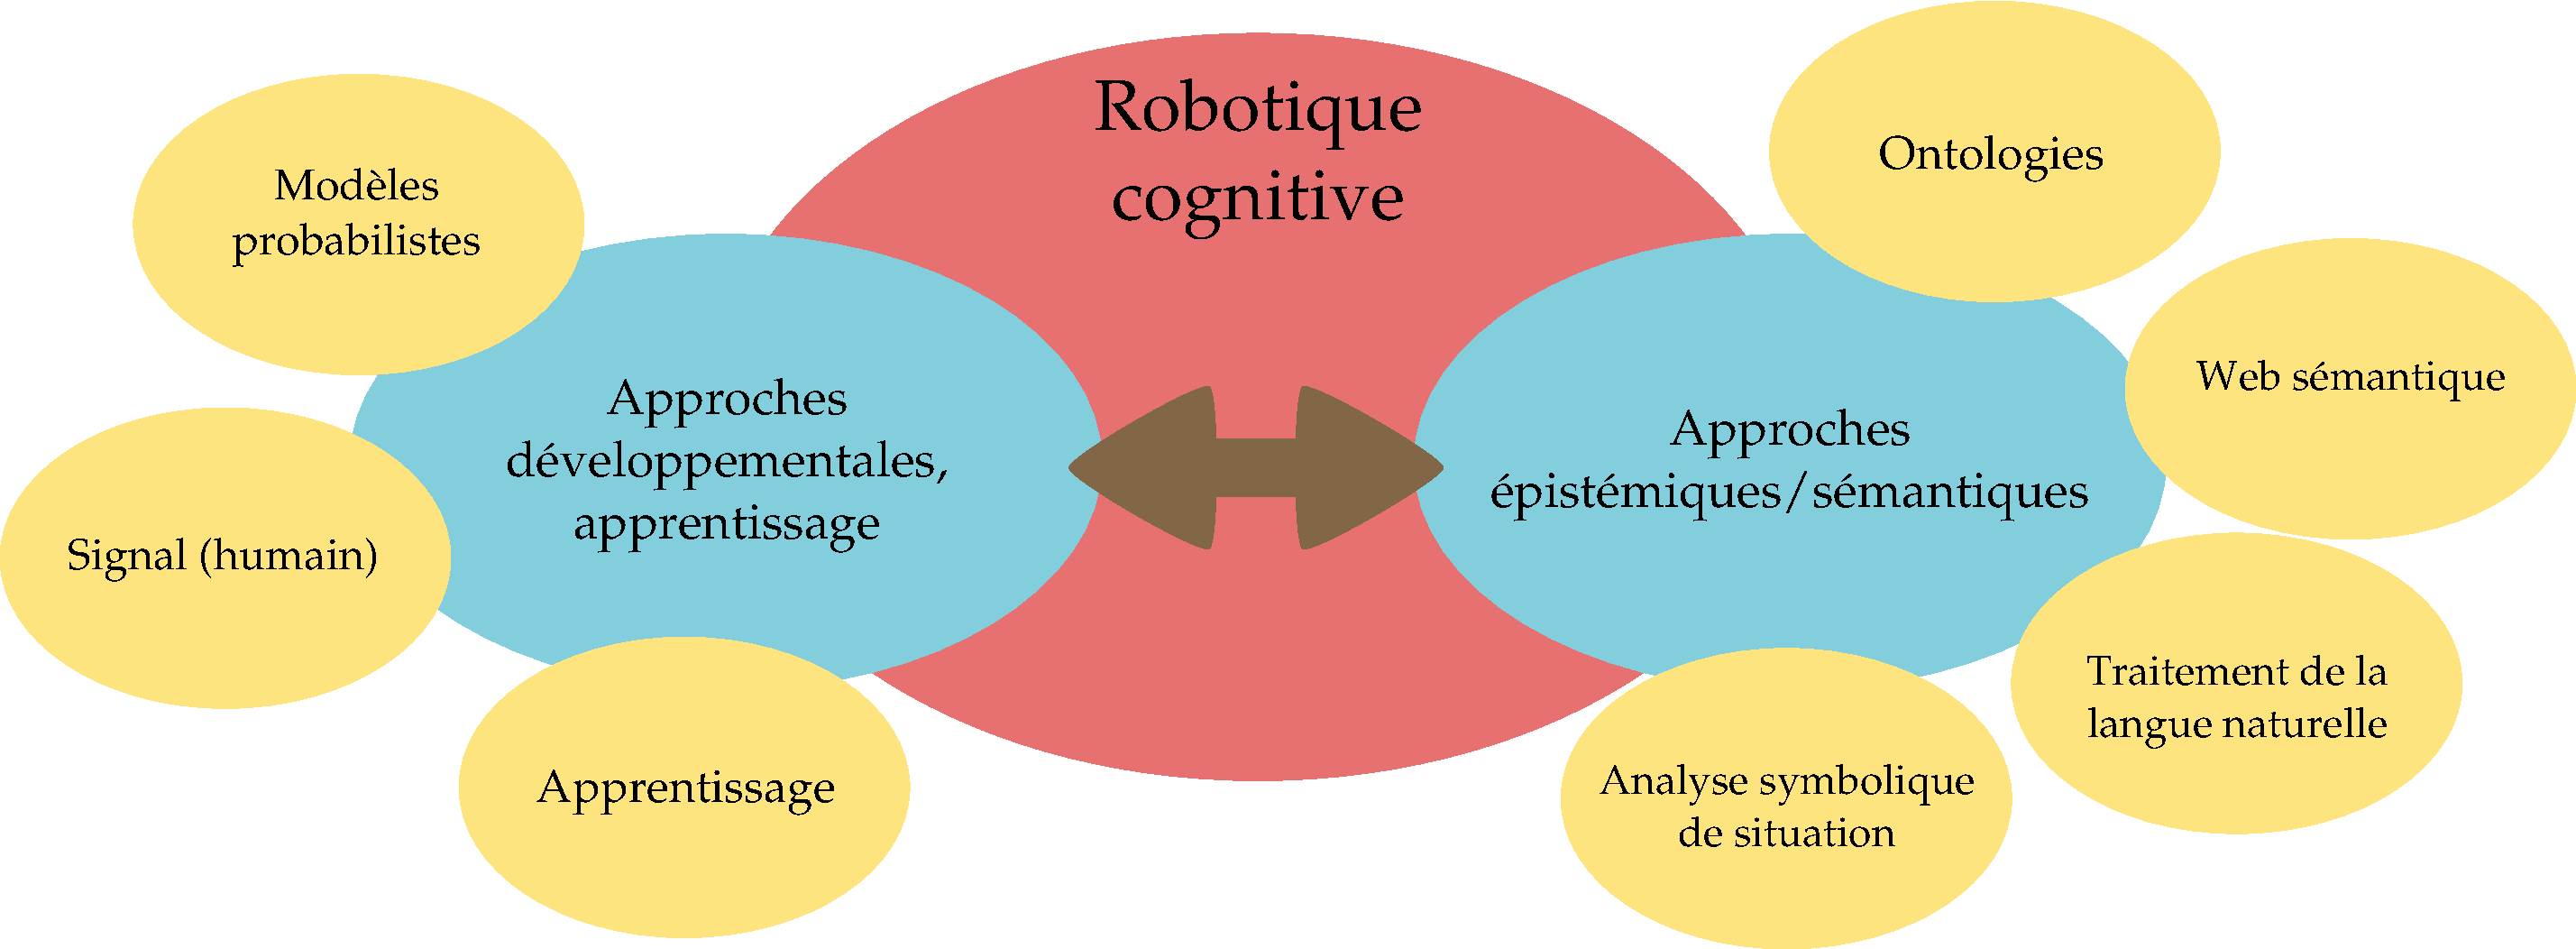
\includegraphics[width=1.0\linewidth]{place}
    \caption{}
    \label{place}
\end{figure}


Deux courants majeurs structurent la recherche en robotique cognitive:
les approches dite épigénétiques ou ancrées d'une part, dans lesquelles
un certains nombre de mécanismes cognitifs émergent ou sont appris par le robot
au contact de son environnement et de ses interactions (en particulier avec les
humains) ; les approches épistémiques d'autre part, dans lesquelles les robots
manipulent des corpus pré-existants de connaissances, et qui travaillent avec des
concepts essentiellement symboliques et abstraits, dont la sémantique est explicite.

Mes activités de recherche antérieures se sont focalisées sur les secondes, dans
un cadre particulier, qui a l'intérêt d'amener des situations riches et complexes
d'un point de vue sémantique : l'interaction homme-robot. Ce choix m'a permis de
mener de premières recherches fructueuses, tant sur la représentation des
connaissances du robot que sur l'implémentation de capacités cognitives
avancées chez les robots (dans le domaine du langage naturel par exemple). Ces
recherches ont été sanctionnées par un prix de thèse en robotique.

Pourtant, ces approches épistémiques et symboliques souffrent d'un manque de
polyvalence et d'adaptibilité. Elles ne sont pas bien adaptées à la
représentation des phénomènes continus ou stochastiques, et ne permettent pas
facilement d'apprendre et de généraliser à partir de situations vécues par le
robot. Ce sont là au contraire les points forts des approches développementales.
Jusqu'à récemment, ces dernières ont cependant souvent été limitées à des
fonctions cognitives simples. Des efforts récents~\cite{morse2010epigenetic,
pezzulo2012computational} tentent de construire un pont entre les deux
approches, en proposant d'employer la robotique cognitive comme
\emph{méthodologie} pour étudier une cognition ancrée et computationelle. Ces
travaux visent en premier lieu à mieux comprendre la cognition \emph{humaine} en
employant le robot comme un support de modélisation.

Le c\oe ur du projet scientifique que je propose se situe de même au carrefour
de ces deux approches, mais garde une perspective essentiellement robotique :
mon objectif est d'accroitre l'autonomie des robots dans des environnements
particulièrement complexes. La problématique que je propose de traiter est ainsi
comment \textbf{mettre en place les ponts entre robotique cognitive
développementale d'une part et épistémique d'autre part, afin de faire
progresser de manière disruptive la qualité et la puissance des modèles
construits et manipulés par les robots, et ainsi, leur autonomie}.

Je propose de plus de poser un cadre de recherche précis pour cette
problématique : l'interaction homme-robot. Je veux y appliquer une double
approche, à la fois \emph{bottom-up} en m'intéressant directement au
\emph{signal humain émis durant l'interaction}, et \emph{top-down} en
définissant a priori un certain nombre de tâches cognitives de haut-niveau que
le robot doit pouvoir maitriser, incluant par exemple un dialogue multi-modal
riche et pertinent ou encore l'implémentation de formes poussées de théorie de
l'esprit.

L'idée maitresse sur laquelle je propose de mener mes recherches est ainsi la
\textbf{combinaison nouvelle de techniques symboliques de type ontologies
ancrées et de techniques d'apprentissage basées sur les signaux humains émis
durant l'interaction homme-robot}. On peut ainsi parler d'\textbf{ontologies
multimodales ancrées}, et à ce titre, ce projet de recherche se situe
au carrefour de la robotique, de la cognition ancrée (``grounded'') qui inclue
des techniques d'apprentissage, et de la cognition symbolique
(figure~\ref{place}).

De manière symétrique, je propose aussi de travailler sur le pendant décisionnel
de cette approche duale cognition ancrée/cognition symbolique en introduisant
une rupture vis-à-vis des approches traditionnelles de type architectures en
couche (contrôle bas-niveau/haut-niveau décisionnel) et architectures
hiérarchiques de type ``subsumption''. L'idée clé est ici de proposer un
\textbf{schéma de décision semi-distribué} où un \textbf{composant cognitif
symbolique orchestre (via des activations et des inhibitions) des boucles
sensori-motrices dites ``réflexes'', construites par apprentissage}.

Mon projet s'articule ainsi en trois axes scientifiques : la recherche de
\textbf{techniques nouvelles permettant de lier signal bas-niveau et modèle
sémantique} ; la conception d'un \textbf{système de représentation unifié,
autour de l'idée d'ontologie multi-modale ancrée} ; la transposition de ces
techniques à la \textbf{décision en robotique, avec la recherche d'une
architecture décisionnelle duale et semi-distribuée}.

Le développement de ces axes est par ailleurs soutenu par \textbf{un programme
expérimental fort}. La menée systématique d'expériences d'interaction en milieux
écologiquement valides reste rare et sujette à des faiblesses méthodologiques.
Dans la continuité de l'expertise que j'ai acquise en post-doctorat, je propose
d'ancrer et de valider mon travail dans un programme expérimental ambitieux, qui
sache ``sortir du laboratoire'' pour se confronter à des environnements
réalistes et complexes.

Ce programme de recherche mêle étroitement robots et humains. Bien que mise en
avant de manière répétée dans les orientations scientifiques européennes (au
sein des \emph{Future and Emerging Technologies} (FETs), les technologies
cognitives sont une des priorités affichées de l'agenda Horizon2020), la
robotique cognitive est relativement peu représentée dans le paysage
scientifique français, les principales équipes de dimensions internationales
étant Flowers, à l'INRIA, et les laboratoires LAAS et ISIR au sein du CNRS. Je
souhaiterais cependant, en premier choix, rejoindre le GIPSA Lab à Grenoble.
Nouveau venu dans le domaine de la robotique, mais de réputation internationale
dans le domaine de l'acquisition et du traitement du signal humain (en
particulier de la parole), il me semble être un environnement remarquable pour
faire progresser la recherche en interaction homme-robot avec des approches
nouvelles et disruptives. Le laboratoire a de plus récemment acquis un robot iCub,
parfaitement adapté à la recherche en interaction homme-robot, et prend depuis
peu une orientation résoluement ``robotique cognitive'', comme le traduit le
nouveau nom de l'équipe ``Cognitive Robotics, Interactive Systems and Speech
Processing'' (CRISSP), anciennement MAGIC.  L'expertise en robotique
d'interaction que je suis susceptible d'apporter s'inscrirait tout à fait dans
cette dynamique.

De plus, d'autres équipes du GIPSA Lab comme l'équipe PCMD (\emph{Parole
Cerveau Multimodalité Développement}) sont spécialistes en cognition et en
psychologie expérimentale, et représentent à ce titre un atout supplémentaire et
renforcent l'intérêt de ce laboratoire pour mener mon programme de recherche.

\subsection*{Axe 1 -- Du signal humain au modèle sémantique}

L'idée de \emph{signal humain} groupe plusieurs dimensions : la familles des
signaux verbaux (parole, dialogue), para-verbaux (uttérances non verbales) et
co-verbaux (gestes accompagnant la parole, attitudes de la voix), le regard
(notamment les mécanismes d'attention conjointe), la posture, et l'ensemble des
gestes déictiques.

Du point de vue de la robotique d'interaction, le traitement du signal humain
soulève deux problématiques principales: comment intégrer ces 
modalités de nature bien différentes, mais étroitement liées ; comment ensuite
transformer ces signaux en une information adaptée et pertinente pour les
processus décisionnels du robot?

[TDB: description technique/algo: modélisation statistique séquentielle ->
(ID)HMM, POMDP...]

[TDB: ...vers le modèle sémantique]

\subsection*{Axe 2 -- Unification des représentations, Application aux fonctions
cognitives}

Le deuxième axe de recherche s'intéresse à l'utilisation effective, en robotique
cognitive, de cette approche continue, du signal au symbole sémantique. Il
s'intéresse d'abord à la question de la représentation \emph{unifiée} des
différentes modalités, ensuite à l'application de cette représentation pour
implémenter de nouvelles compétences cognitives supérieures chez les robots. Je
propose de focaliser cette recherche sur le domaine de la modélisation mutuelle
homme-robot : comment le robot peut construire un modèle cognitif des
connaissances et croyances de l'homme. Ceci pour donner au robot une
\emph{théorie de l'esprit} au niveau des \emph{représentations} et non pas
uniquement des perceptions, ce qui représente une avancée notable de l'état de
l'art dans le domaine de la robotique socio-cognitive.

\subsubsection*{Système de représentation}

\begin{figure}
    \centering
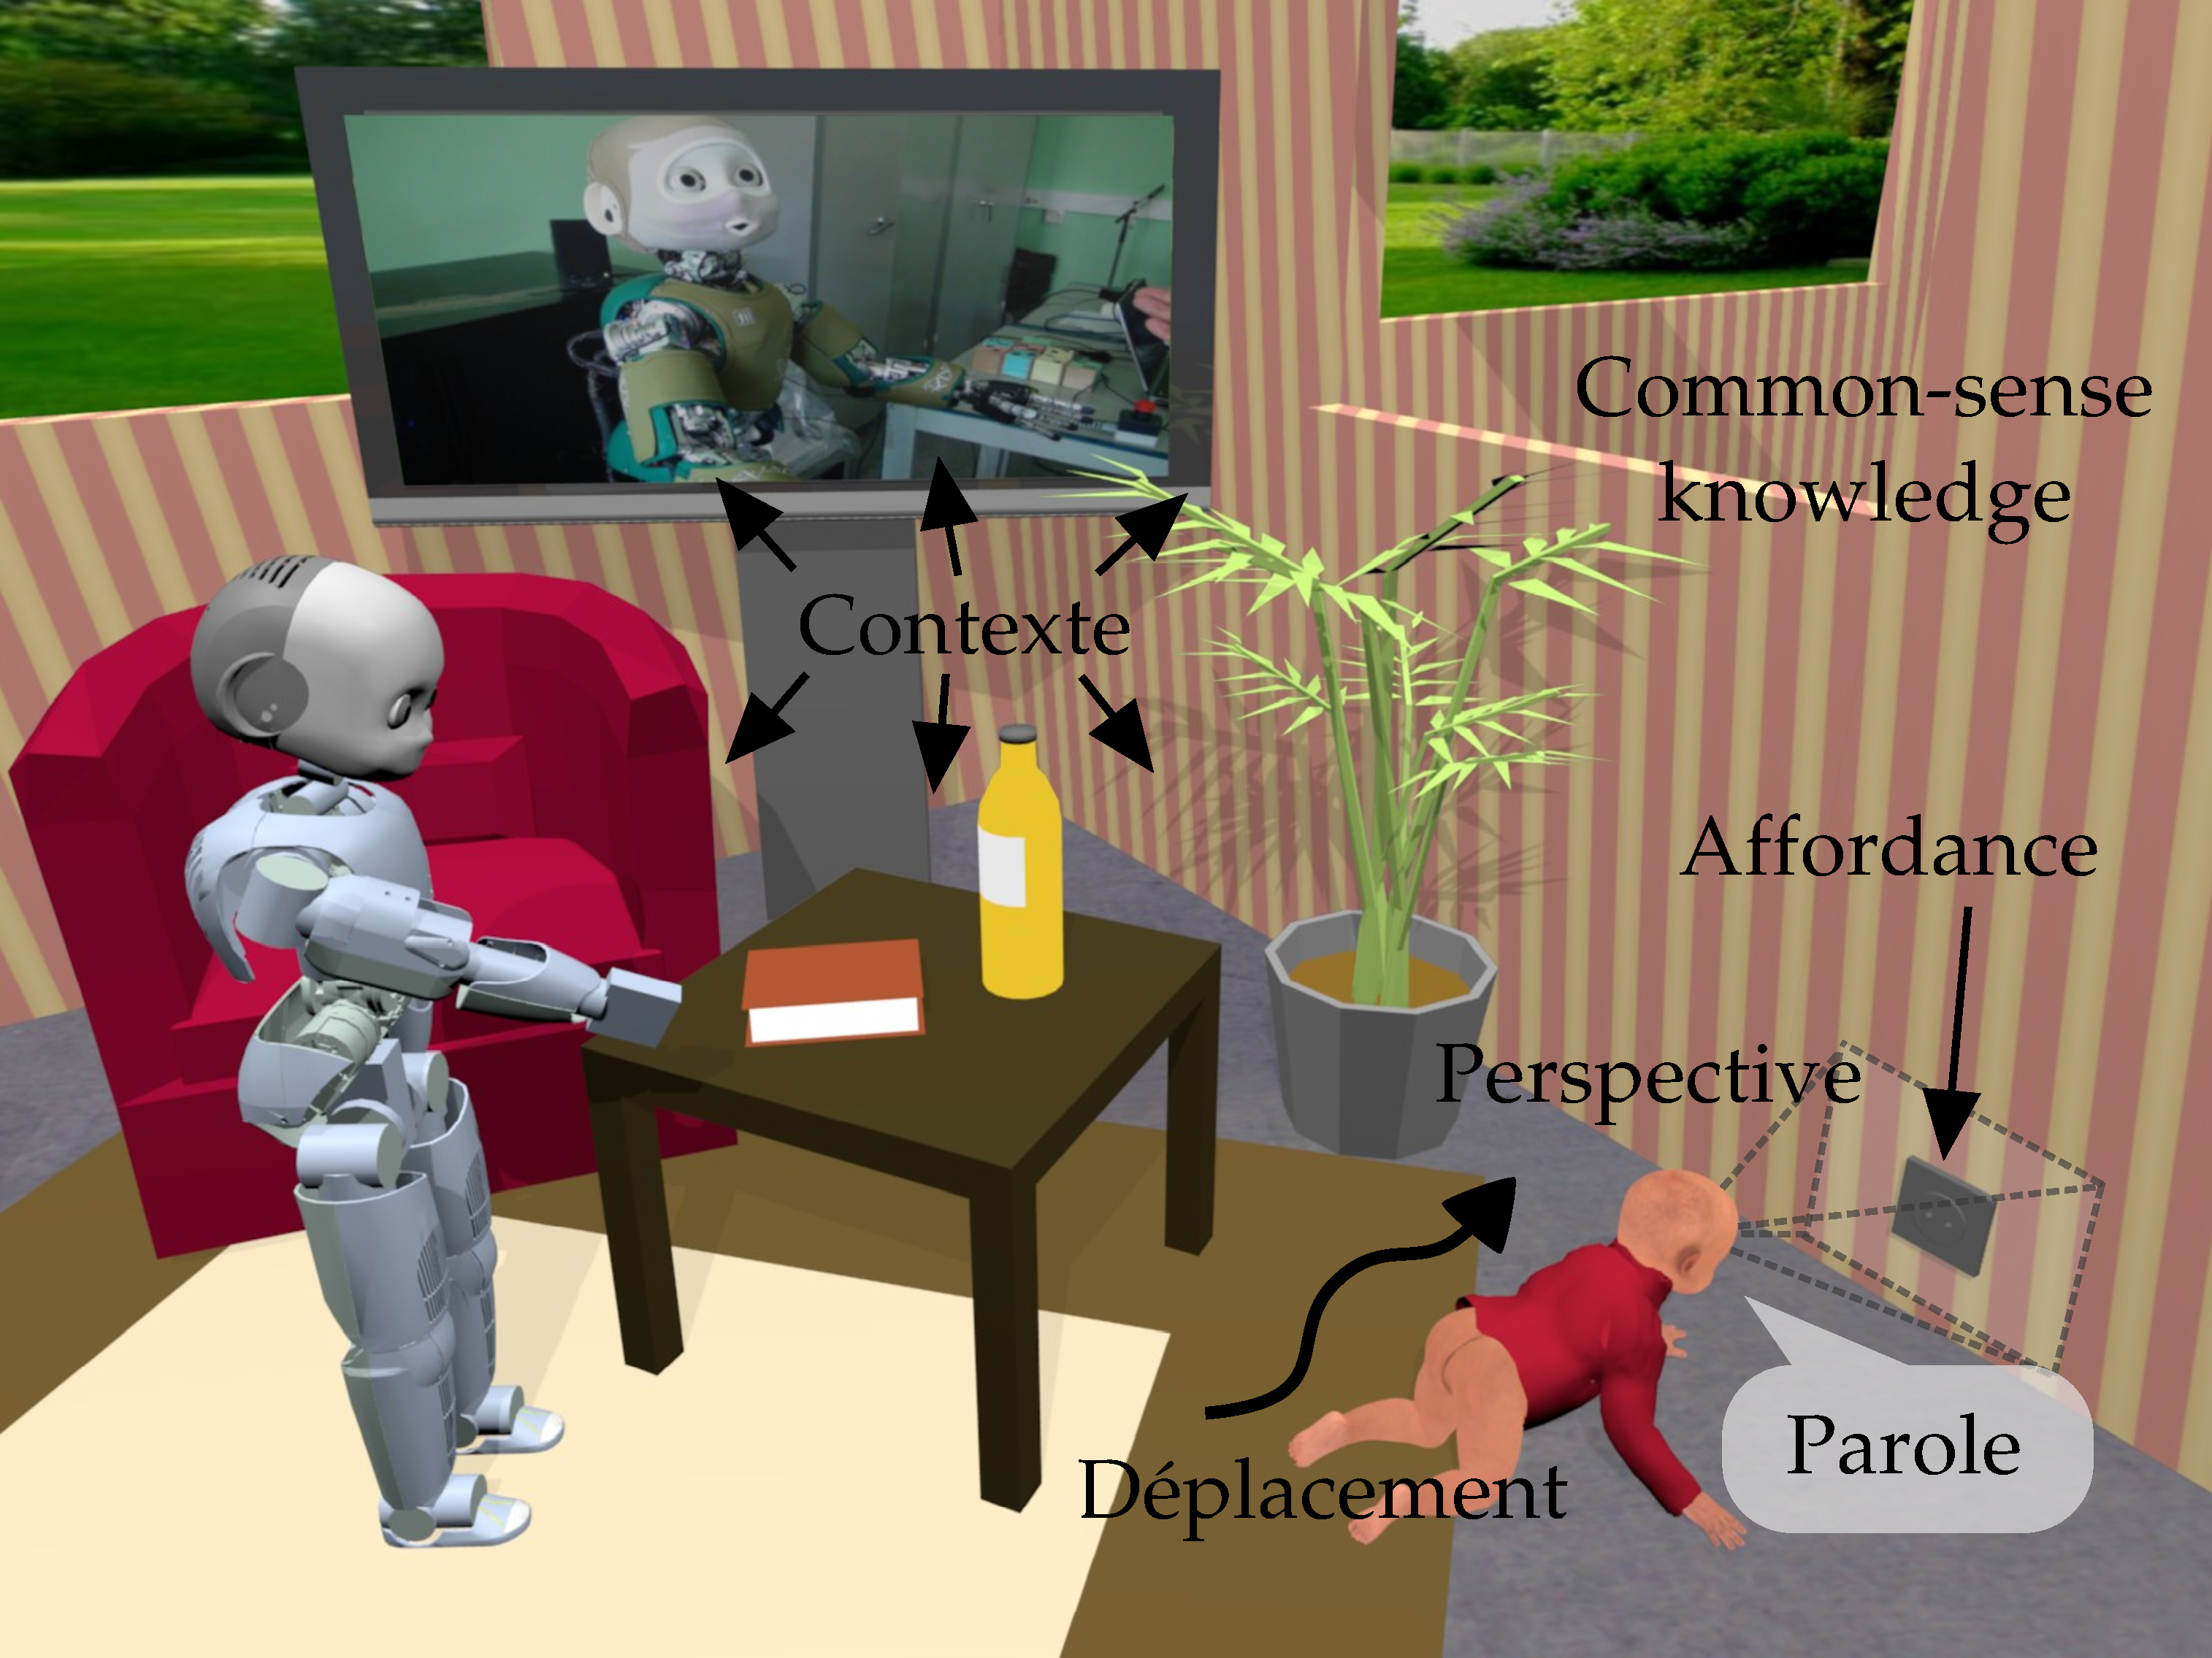
\includegraphics[width=0.7\textwidth]{figs/signaux}
\caption{\small Pour comprendre ce type de situation, il est
    nécessaire de construire une représentation \emph{unifiée} de
    l'environnement, incluant un modèle géométrique, un modèle de l'humain
    construit à partir des signaux qu'il émet, un modèle
    sémantique (qui inclue une représentation des affordances), un modèle
    temporel (qui puisse aussi être utilisé comme modèle prédictif), et enfin,
    un modèle des croyances et intentions de l'humain.}
\label{babyplug}
\end{figure}

Le travail que j'ai mené durant mon doctorat m'a amené à analyser huit systèmes
de représentation des connaissances effectivement déployés sur des robots. Un
point clé de comparaison de ces systèmes est leur approche de l'ancrage
symbolique (\emph{symbol grounding}) dans leur environnement physique, et il en
ressort que la capacité pour un robot à représenter son environnement de manière
(au moins partiellement) symbolique est à la
fois la pierre angulaire de ses capacités cognitives supérieures (raisonnement,
prise de décision, communication) et un défi qui n'est pas aujourd'hui traité
dans toute son ampleur.

Les recherches actuelles sont essentiellement focalisées sur la représentation
géométrique de l'environnement du robot. La construction en ligne de
cartes sémantiques~\cite{Nuechter2008, Galindo2008,
Blodow2011} ou l'utilisation d'affordances fonctionnelles~\cite{Varadarajan2011}
sont des exemples de l'état de l'art au regard de la construction de liens
géométrique-symbolique sur l'environnement spatial du robot.

De même, le travail sur une représentation \emph{amodale} de
l'environnement~\cite{Mavridis2006}, prenant en compte les incertitudes et
permettant de représenter des entités spatiales non-vues (donc de les imaginer),
apporte plusieurs idées importantes, mais se cantonne essentiellement aux
aspects spatiaux.

La représentation de l'environnement temporel du robot a aussi fait l'objet de
recherches (avec les idées de \emph{chroniques}~\cite{Ghallab1996}, les
approches par \emph{fluents}~\cite{mosenlechner2010becoming}, l'idée
d'\emph{instantanés}~\cite{Mavridis2006}), mais la plupart de ces travaux
s'apparentent à une journalisation des événements, accompagnée d'outils
d'analyse et d'apprentissage (en général hors-ligne). Ni la possibilité de
naviguer naturellement dans les états antérieurs, ni la création et la
représentation d'états futurs hypothétiques ne sont intégrées au niveau d'une
représentation globale de l'environnement du robot.

Quant à l'intégration de la représentation d'affordances, de contextes (en
particulier, de contextes sociaux, comme dans la figure~\ref{babyplug}), de
modèles de croyances et d'intentions, le travail reste largement à faire (on
peut toutefois mentionner la représentation de différentes perspectives, comme
dans~\cite{ros2010which}). Le premier de ces défis étant d'ailleurs de concevoir
une modalité de représentation pour les affordances, contextes, croyances qui
puisse être unifiée dans un modèle de l'environnement.

Cette axe de recherche, qui prend son point de départ dans mon travail de
post-doctorat au LAAS, vise à faire progresser l'état de l'art dans le domaine
de l'ancrage symbolique en proposant de concevoir et d'implémenter une
représentation unifiée de l'environnement du robot, fusionnant les modèles
continus (modèles géométrique, historique des évènements, etc.) et les modèles
symboliques (connaissances symboliques générales sur le monde, croyances des
agents, affordances, etc.). Je conçois ce modèle de l'\emph{Umwelt} du robot (le
monde \emph{perçu}, \emph{propre} du robot) comme une brique importante devant
servir de support pour le développement et l'intégration d'architectures
décisionnelles pour les robots.


\cite{pezzulo2012computational} -> p5: modal vs amodal representation -> ``zones
de convergences'' des représentations chez [Damasio, 1989] et [Simmons et Barsalou,
2003].

\subsubsection*{Modélisation mutuelle homme-robot}

Comme je l'ai présenté dans~\cite{lemaignan2014human}, si la robotique
cognitive, qui hérite à ce titre de la psychologie cognitive, s'intéresse aux
processus mentaux comme l'\emph{attention}, l'utilisation du \emph{langage}, la
\emph{mémoire} ou les processus de \emph{prise de décision}, la cognition
sociale y ajoute les aspects lié à la prise en compte des interactions avec
d'autres agents : \emph{représentation des croyances}, \emph{prise de
perspective}, \emph{action conjointe}, et tous les aspects liés à la
\emph{communication}.

Les dynamiques sociales humains s'appuient sur la capacité à attribuer de
manière pertinente des croyances, des buts et des percepts aux autres. Cet
ensemble de capacités meta-représentationelles forment ce qu'on appelle une
théorie de l'esprit, et conduit à la modélisation mutuelle : la capacité
réciproque d'établir un modèle mental de l'autre. Ceci se retrouve au c\oe ur
des interactions humains : une interaction sociale normale dépend de la
reconnaissance de perspectives sensorielles différentes, de la compréhension
d'états mentaux différents, et de la reconnaissance d'indices attentionels et
émotionels non-verbaux complexes. Transférer de telles compétences cognitives aux
robots sociaux apparait ainsi comme un objet de recherche important en
interaction homme-robot.

Cependant, jusqu'à présent, la communauté de l'interaction homme-machine n'a
qu'effleuré cette question : Scassellati donnait en 2002
dans~\cite{scassellati2002theory} un premier aperçu des modèles de Leslie et
Baron-Cohen de la construction d'une théorie de l'esprit du point de vue de la
robotique, sans réelle implémentation. Depuis, la recherche dans ce domaine
s'est essentiellement focalisée sur des applications de prise de perspective
(``\emph{je vois que tu ne vois pas le livre}''), utilisant la vision comme
principale (souvent unique) modalité sensorielle. Les principaux travaux sur
cette questions sont par Breazeal~\cite{breazeal2006using},
Trafton~\cite{Trafton2005} et Ros~\cite{Ros2010} (j'ai étroitement travaillé
avec cette dernière sur ces questions).

\begin{figure}[h!t]
        \centering
        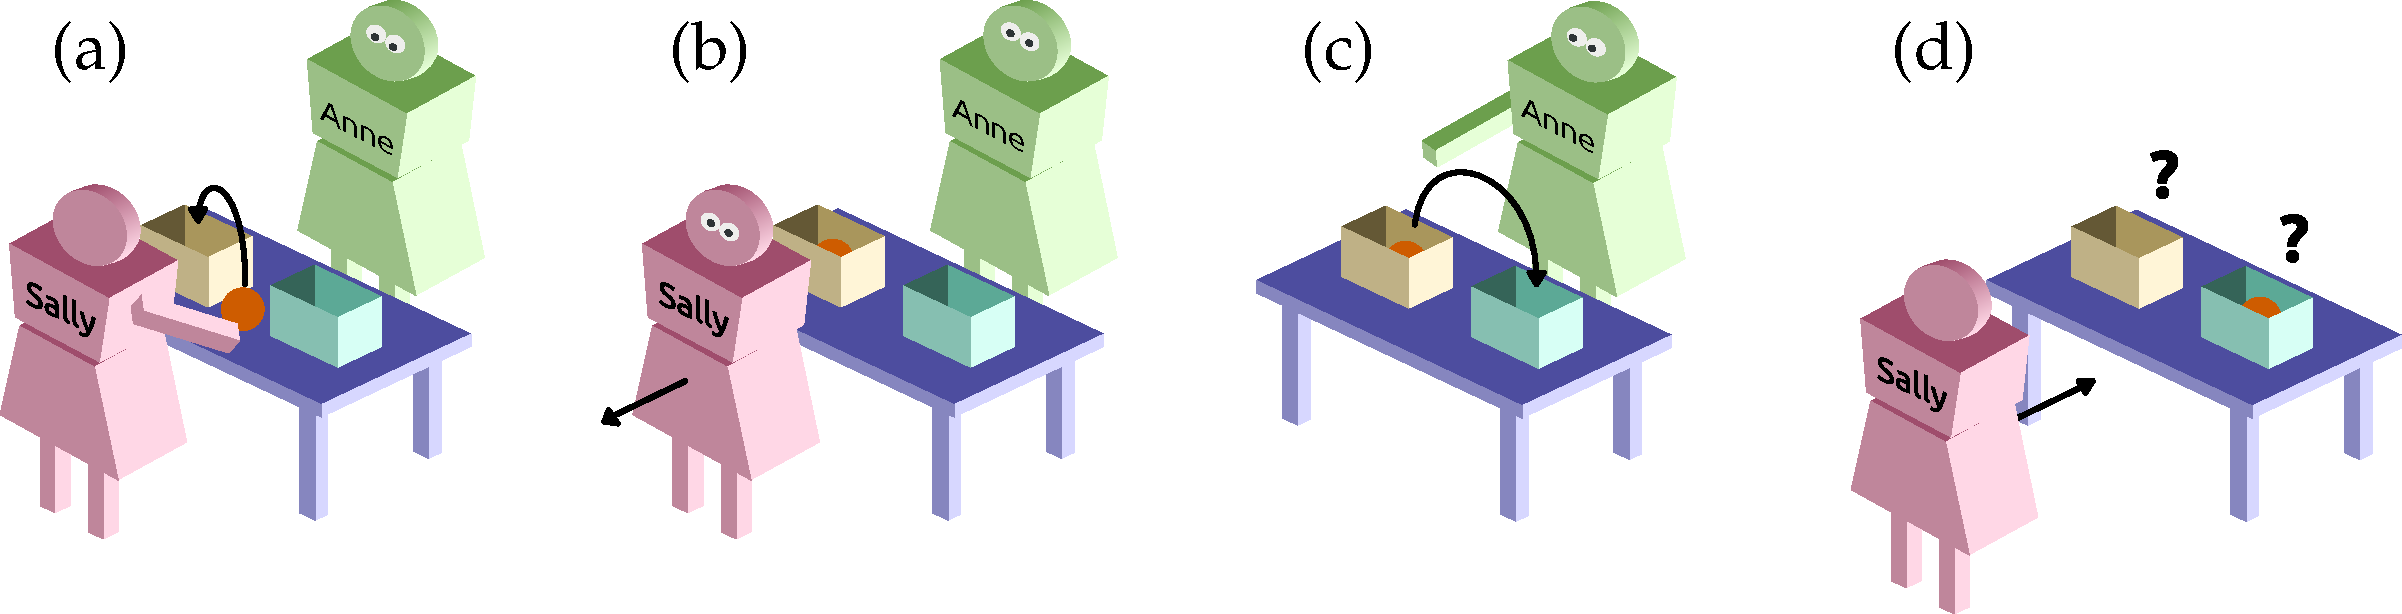
\includegraphics[width=0.7\linewidth]{sally_ann}
        \caption{\small L'expérience de ``False belief'': deux poupées, Anne
            et Sally, se font face, avec deux boites entre elles. Un enfant
            (le sujet) observe la scène. Sally place une balle dans la boite
            beige, puis s'en va. Anne déplace la balle dans la boite bleue, puis
            Sally revient. L'expérimentateur demande à l'enfant: \emph{Où
            penses-tu que Sally va aller chercher la balle ?}. Sans une théorie
            de l'esprit (\ie, avant 3-4 ans), l'enfant n'est pas capable de
            projeter des croyances fausses dans le modèle mental de Sally, et se
            trompe en répondant \emph{Dans la boite bleue}. En terme de
            représentations, une prise de perspective visuelle suffit pour
            réussir cette tâche.}
        \label{false-beliefs}
\end{figure}

En se basant sur une prise de perspective uniquement visuelle, Breazeal
\etal\cite{breazeal2009embodied} et Warnier \etal\cite{warnier2012when} (travail
auquel j'ai participé) ont pu implémenter le test classique de théorie de
l'esprit, l'expérience de Sally et Anne (figure~\ref{false-beliefs}, introduite
par Wimmer~\cite{wimmer1983beliefs}, protocole expérimental par
Baron-Cohen~\cite{baron1985does}). Ils ont pu faire la démonstration de systèmes
complets dans lesquels le robot reconnait et prend en compte des
situations de croyances fausses durant des interactions dyadiques ou triadiques,
et met en \oe uvre des comportements permettant d'aider le partenaire humain en
fonction des connaissances manquantes ou fausses de celui-ci.

Ces résultats sont importants et rassurant quant à la possibilité de doter les
robots de compétences socio-cognitives avancées. Intuitivement, on voit
cependant aussi que la modélisation mutuelle ne se résume pas au calcul de ce
que l'humain voit ou ne voit pas. Les perceptions se traduisent en
représentations subjectives : comment pouvons nous y accéder ? comment mesurer
ce que l'autre sait de moi-même ? les modèles mutuels se superposent à l'infini
en ``Je sais que tu sais que je sais...'' : comment les représenter et
les manipuler ? Se pose aussi la question de la dimensionalité de ces modèles :
doivent-ils être locaux à la tâche en cours, ou plus généraux ? Comment
différencier une réelle modélisation cognitive d'une simple imitation durant une
action conjointe ? Toutes ces questions soulingent la complexité d'un mécanisme
cognitif dont l'étude se situe au croisement de plusieurs champs académiques. La
robotique, en tant que science de l'intelligence artificielle incarnée, peut et
doit être le point de convergence pour valider notre compréhension de cette
compétence socio-cognitive.

\subsection*{Axe 3 -- Décision distribuée et architecture cognitive pour l'interaction homme-robot}

[TDB: A faire! développer vers l'idée de décision distribuée -- boucle
sensori-motrices]

L'idée de \emph{robotique cognitive} n'est pas récente (elle est mentionnée dès
le début des années 1990 par Reiter~\cite{Levesque2008}), et est déjà établie
comme un champ de recherche actif, formant le pendant des approches
développementales de la robotique. Si ce domaine n'est pas nouveau, il est
cependant traité de manière essentiellement atomique en robotique : les
compétences cognitives sont implémentées et testées indépendamment les unes des
autres, et comme le note Kurup~\cite{kurup2012what}, ce n'est que récemment que
la robotique s'intéresse aux architectures cognitives holistiques développées en
intelligence artificielle. Les travaux de Chen~\cite{Chen2010}, de
Beetz~\etal~\cite{Beetz2010}, de Trafton~\etal sur
ACT-R/E~\cite{trafton2013act}, les recherches menées par Baxter dans le cadre du
projet européen ALIZ-E~\cite{baxter2013cognitive} et les travaux du
LAAS-CNRS~\cite{lemaignan2014human} en sont les principaux exemples récents.



~\cite{morse2010epigenetic}

~\cite{baxter2013cognitive}: cognition as a memory activation issue, amorçage, importance
de l'alignement comportemental entre partenaires d'une interaction
%ACT-R/E est un exemple intéressant dans la mesure où l'architecture est conçue
%en premier lieu pour l'interaction homme-robot, et elle est évaluée en se
%référant explicitement à la psychologie développementale. Elle illustre aussi le
%chemin qui reste à parcourir dans ce domaine : bien qu'étant une architecture
%cognitive globale, elle n'a été testée que sur des compétences cognitives
%isolées, en laboratoire, et ignore largement les problématiques d'ancrage
%symbolique (le robot raisonne sur un environnement simplifié, et les modalités
%de communication sont elles aussi simples -- pas d'interaction linguistique, par
%exemple).

\begin{figure}
    \centering
    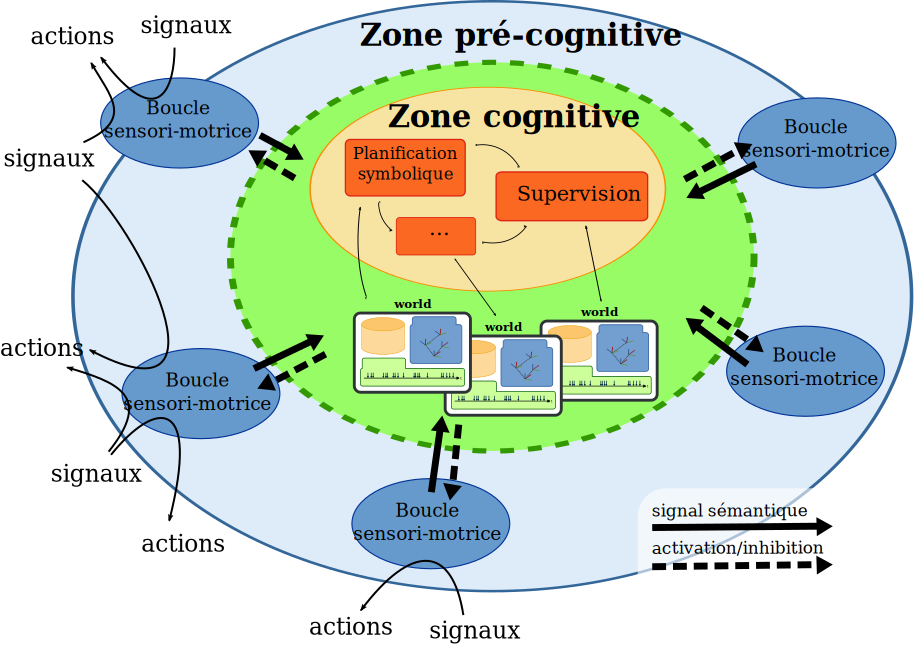
\includegraphics[width=0.8\linewidth]{archi}
    \caption{\small Intégrer un contrôle cognitif explicite avec des boucles
        sensori-motrices ``réflexes'', dites \emph{pré-cognitives}, au sein
    d'un nouveau type d'architecture cognitive pour les robots d'interaction.}
    \label{}
\end{figure}


Mais de manière générale, encore peu de travaux s'intéressent à l'étude des
architectures cognitives dans le cadre spécifique de l'interaction homme-robot,
qui synthétise beaucoup des défis de la robotique : environements dynamiques dont la
sémantique est complexe, suivi et représentation de l'homme, action conjointe,
nécessité d'une grande réactivité pour assurer une interaction de qualité.

J'ai montré
durant mon doctorat qu'il était possible de construire et d'exploiter en ligne
des modèles cognitifs riches des autres agents, et d'intégrer ces modèles dans
la prise de décision~\cite{alami2011when, warnier2012when, lemaignan2014human}.
Pour autant, une traduction systématique de mécanismes de cognition sociale en
terme d'architecture décisionnelle est une question essentiellement ouverte. La
prise en compte de codes et comportements sociaux implicites (ébauchée au niveau
de la planification symbolique dans des travaux comme~\cite{Alili2009}) ou
l'analyse d'environnements particulièrement riches en terme de sémantique (comme
l'illustre la figure~\ref{babyplug}) sont des exemples des spécificités de
l'interaction homme-robot qui ont un impact important sur la conception d'une
architecture de contrôle.

Ce troisième axe de recherche vise non seulement à bâtir les ponts nécessaires
entre les approches théoriques et fondamentales des deux précédents axes d'une
part, et les applications expérimentales de cette recherche d'autre part. Il
s'agit aussi d'implémenter et d'organiser de manière formelle un nombre élevé de
mécanismes cognitifs ego- \emph{et} allocentrés en une architecture complète et pertinente, apte à être
déployée sur des robots d'interaction autonomes.

\subsection*{Programme expérimental}

En me basant sur mon expérience acquise dans la menée d'expérience d'interaction
homme-robot en environnements écologiques~\cite{lemaignan2010oro,ros2010which,lallee2011towards,lemaignan2012roboscopie,warnier2012when,hood2015when}, y compris avec des robots
complexes type PR2,
je propose de matérialiser les axes de recherche que j'ai présenté sous la forme de
plusieurs objectifs expérimentaux, à la fois en laboratoire et sur le terrain.
Une première série d'expériences vise à démontrer l'intérêt d'une représentation
unifiée de l'environnement du robot pour développer des capacités cognitives
nouvelles ; une série d'expériences suivante s'intéresse à l'utilisation de ces
capacités nouvelles dans des scénarios d'interactions complets.  Ce
programme expérimental vise à faire avancer significativement l'état de l'art en
ce qui concerne la robotique d'interaction, aussi bien en terme algorithmique,
qu'en terme d'intégration concrète et d'usages en situation réelle.


Je propose dans un premier temps de recréer en laboratoire un ensemble de
situations d'interaction dans l'esprit de la figure~\ref{babyplug}: de court
(~ 10 min) épisodes
de la vie courante impliquant robots et humains dans des tâches réalistes de
reconnaissance de situation et de manipulation d'objets, et pour lesquelles une
interprétation correcte nécessite de combiner représentations multi-modales
ancrées et représentations sémantiques, d'être capable de construire un modèle
fin de l'homme, incluant la reconnaissance de séquences d'actions, et de
reconnaitre et mobiliser l'ensemble des contextes de l'interaction. La qualité
et la pertinence des modèles et de l'interprétation de la scène réalisée par le
robot est ensuite évalué en les comparant aux interprétations produites par des
observateurs humains dans le même contexte.

Je prévois ensuite une seconde famille d'expériences s'intéressant à la prise de
perspective au niveau des \emph{représentations} : il s'agit de tester la
capacité du robot à construire un modèle des représentations \emph{abstraites}
des autres, et je propose d'explorer cette question à travers l'idée de
\emph{tromperie adaptative} : dans une séquence de jeu, le robot à la
possibilité de \emph{mentir} (\ie, de tromper son partenaire) afin de renouveler
l'intérêt ludique et de maintenir l'engagement d'autre joueur. Le choix de
mentir à un instant donné sur base sur la représentation (telle qu'estimée par
le robot) qu'à le joueur de la situation courante. Un exemple d'une situation
de jeu se prêtant à cette idée de \emph{tromperie adaptative} est le protocole
en psychologie expérimentale du \emph{Penny Hiding Game} (protocole initialement
proposé par Oswald and Ollendick~\cite{oswald1989role}, et répliqué et étendu
par Baron-Cohen dans~\cite{baron1992out}) : un joueur cache dans une main un
objet, et l'autre joueur doit deviner la main. Après quelques essais, des
stratégies de jeu se mettent en place pour tromper l'adversaire et l'inciter à
choisir la main incorrecte. Dans un tel scénario, le robot peut adapter cette
stratégie de jeu en fonction de ce qu'il perçoit du comportement, et
indirectement, des représentations, de l'autre joueur.

%La troisième expérience s'intéresse à la fois au déploiement d'une architecture
%cognitive pour l'interaction en autonomie, et aux facteurs cognitifs d'une
%interaction de longue durée. L'objectif est de déployer des robots de type Nao avec
%des schémas d'interaction restant simples (tâches du type lecture de recette ou
%d'histoire pour les enfants) dans des familles non-expertes, et sur des
%périodes longues (de l'ordre de 3 mois). Cela vise à acquérir et valider les
%facteurs, tant humains que robotiques, qui permettent d'établir un engagement
%durable.  Je souhaite échelonner plusieurs déploiements dans plusieurs familles
%en parallèle, et cette expérience pourrait s'étaler de J+24 mois à J+30 mois.
%
%Enfin, en s'appuyant sur les enseignements issus de l'expérience précédente, le
%dernier objectif expérimental, plus ambitieux, consiste à déployer un robot
%complexe type PR2, dans une famille, pour une durée longue, et avec un
%répertoire d'interactions étendu, incluant autonomie complète, dialogue
%multi-modal, manipulation conjointe. Je situe cet objectif expérimental à un
%horizon J+36 mois. Au-delà du défi scientifique que cela représente (il
%s'agirait d'une première internationale), cette expérience aurait probablement
%un impact sociétal, et représenterait à ce titre une étape dans la recherche en
%interaction homme-robot.
%

\subsection*{Conclusion}

[TDB: a faire]

%
%En paraphrasant McCarthy, on peut dire de ce projet de recherche qu'il s'inscrit
%dans le programme (à long terme) d'une ``intelligence incarnée de niveau
%humain''. Il se positionne sur la question particulière de \emph{l'intelligence
%sociale} dans le contexte d'interactions entre agents artificiels physiques et
%humains.
%
%Je propose dans un premier temps de poser des bases rigoureuses, qui semblent
%aujourd'hui manquer, à l'analyse et l'évaluation des performances cognitives des
%robots, en particulier dans ce contexte social.
%
%Je propose ensuite d'attaquer la question de la fusion des représentations
%multiples de l'environnement du robot, parfois continues, parfois symboliques,
%en un modèle unifié. Ce modèle doit de plus intégrer des dimensions nouvelles
%(contextes, affordances, modèles de croyances des différents agents), et
%construire ainsi des fondations solides pour les processus cognitifs supérieurs.
%C'est une question de recherche aujourd'hui ouverte, qui fait appel à des
%techniques de représentations hybrides qui sont à découvrir.
%
%Sur cette base, je propose de travailler sur l'intégration de mécanismes
%cognitifs multiples au sein d'une architecture logicielle pertinente pour un
%robot d'interaction. C'est ici au contraire un travail de synthèse, qui
%s'appuie, en le développant, sur le corpus scientifique existant, tant en
%robotique qu'en intelligence artificielle (architectures cognitives), qu'en
%sciences et neuro-sciences cognitives (modèles décisionnels humains).
%
%Enfin, parce que la recherche en robotique a aussi cette spécificité d'être une
%science de l'intégration technologique, je propose d'organiser mon travail de
%chercheur autour d'objectifs expérimentaux ambitieux, qui puissent aussi donner
%à voir et à réfléchir sur l'impact de la recherche sur la vie de tous les
%citoyens.
%
\printbibliography

\end{document}
